\chapter{Introduction}\label{chapter:introduction}

\section{What is Game Theory?}

A common definition of the subject is:

\begin{quote} 
``Game theory is the study of interactive decision-making where
the outcomes of one decision maker’s choices depend on the decisions made by
others.'' 
\end{quote}

While this definition captures the essence of strategic interaction, game theory
is much more than that. It is a beautiful mathematical discipline with deep
theoretical avenues for exploration. It plays a crucial role in the global
economy, with multiple Nobel Prizes awarded for contributions to our
understanding of markets. It provides models that explain how biological
structures, from cells to ecosystems, evolve over time. It offers insights into
cooperation, competition, and the formation of social norms.

Because game theory spans multiple disciplines, no single definition fully
captures its scope. This book aims to provide a solid understanding of game
theory—what it can do and how to apply it.

\section{Who is this book for?}

This book is written primarily for advanced undergraduate mathematicians and
computer scientists. It may also serve as a starting point for early-career
researchers seeking a practical understanding of game theory.  

However, the book aims to be accessible to aspiring game theorists from any
discipline. A psychologist modeling a specific behavior? A conservationist
analyzing the conditions under which a policy is likely to succeed? An economist
studying strategic interactions in competitive markets? A computer programmer
implementing a game-theoretic algorithm? Whatever your background, this book
provides the necessary tools to engage with game theory in a meaningful way.  

The book includes four chapters that introduce mathematical theory independently
of game theory. For some readers, these may serve as a review of familiar
topics, while for others, they offer a first introduction to key techniques
needed to apply game-theoretic ideas effectively.  

Game theory is a field that thrives on cross-disciplinary insights, and this
book is designed to help readers from different backgrounds develop a shared
mathematical foundation. Whether your interest is theoretical or applied, the
goal is to equip you with the tools to explore game theory with confidence.  

\section{How is this book different from similar books?}

There are a number of excellent books on game theory that are highly
recommended. For a fantastic introduction to the topic aimed at a mathematical
audience, see~\cite{webb2007game}. The exhaustive work~\cite{maschler2020game}
offers a vast amount of breadth and depth on the subject,
while~\cite{roughgarden2010algorithmic} delves into modern algorithmic
approaches to modeling complex systems at an advanced level.

Some excellent texts focus on specific subtopics within the domain. For
example,~\cite{gusfield1989stable} explores matching games,
and~\cite{roughgarden2002selfish} addresses routing games. Other great general
introductions include~\cite{osborne2004introduction},~\cite{watson2002strategy},
and~\cite{gusfield1989stable}, to name just a few.

This book, however, offers something that these fantastic works do not: detailed
implementation instructions, including multiple examples and exercises that show
how to solve specific problems, even when they are large and complex.
Additionally, it provides an overview of open-source software tools that are
readily available to solve real-world problems. The book also includes case
studies demonstrating how game theory can be applied in practice. Finally, it
offers a rigorous theoretical foundation, serving as a springboard for deeper
theoretical analysis.

\section{How is this book organised?}

\section{How is this book organised?}

Each chapter in this book follows a structured format:

\begin{enumerate}
    \item  \textbf{A motivating case study:} a running example throughout the chapter to 
        illustrate and contextualize the theory, often drawing from real-world scenarios.
    \item  \textbf{Relevant definitions and theory:} providing a rigorous mathematical 
        foundation for the chapter’s topic.
    \item  \textbf{Exercises:} a range of problems inviting the reader to apply the definitions 
        and theory to deepen understanding.
    \item  \textbf{Practical implementations:} including pseudocode, Python code, and an 
        overview of relevant open-source tools to guide implementation.
    \item  \textbf{Contemporary research:} a hand-picked, non-exhaustive overview of 
        relevant research related to the chapter.
\end{enumerate}

Some readers may prefer to focus on the theoretical foundations, while others
might engage primarily with the case studies and practical implementations. This
book is designed to be flexible, allowing readers to approach the material in a
way that best suits their background and interests.

Figure~\ref{fig:structure} shows the general structure of the book and how the
various chapters link together.

\begin{figure}[!htbp]
    \newcommand{\imagenode}[3]{ % #1 = Chapter label/dir, #2 = position, #3 Chapter title
            \node (#1) at #2 [label=above:\raisebox{-3em}{{\parbox{4em}{\centering \tiny #3}}}] {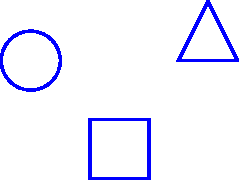
\includegraphics[width=4em]{chapters/#1/logo/main.pdf}};
    }
    \begin{center}
        \begin{tikzpicture}[
                every node/.style={draw, rounded corners=5pt, minimum size=1.5cm, inner sep=5pt},
                every path/.style={thick}
            ]


            % First row of chapters
            \imagenode{normal_form_games}{(-3, 1)}{Chapter 1: Normal Form Games}
            \imagenode{strategies}{(-3, -3)}{Chapter 2: Strategies}

            % Edges showing relationships
            \draw[->] (normal_form_games) to [out=-135, in=135] (strategies);

        \end{tikzpicture}
    \end{center}
    \caption{Visual representation of the relationships and flow between chapters.}\label{fig:structure}
\end{figure}
